\chapter{Results}
\label{chap:results}

\section{Summary}
Sensitivity testing on benchmark P3HT morphology provided by the Evan and matty work can was finegrained and
used to compare to previous mobility results as well as to test the senesitity of the algorithm to
rorganzation energy, dcut, MSD calculation, and siulation temperature.

On the spot MD simulation of 1000
molecules was performed for testing morph another benchmark OPV material. Janks/mattys work has shown that taking
each monomer to be a chromophore even though charges are known to delocalize on 7 monomers still reproduces
the overall mobility well because the very fast hops along the backbone. I think the application of this
hopping model to ITIC other small molecules is even more justified. Knowing that the this molecule has
negligible electron density in the side chains, chomophores are taking to be the backbone. The effect that
the side chains have on mobility aren't a result of the an electronic contributiom to the frontier molecular
orbitals but rather is a result of the effect the chains have on the morphology of the material. 

Delineating chromophores within a morphology needs to be justified by DFT or expirement and balanced against
the computational costs. Furthermore, in this workflow, manually indexing the atoms of the chosen chromophore
remains a significant hurdle. Tutorials on github show how to use the open source tool VMD to speed up this
leg of the worflow. We have also had success with Grits and smarts matching to delineate chromophores through
out the morphology. 

\subsection{Accuracy}

\begin{table}[ht]
    \caption{Mobility $cm^{2}/Vs$} % title of Table
\centering % used for centering table
\begin{tabular}{c c c c} % centered columns (4 columns)
\hline\hline %inserts double horizontal lines
Software & Amorphous & Semi-crystalline & Crystalline \\ [0.5ex] % inserts table
%heading
\hline % inserts single horizontal line
    ORCA & $0.1085 \pm 0.0006$ & $0.0156 \pm 0.0003$ & $0.123 \pm 0.001$ \\ % inserting body of the table
PySCF & $.0018 \pm .000001$ & $.00148 \pm .000001$ & $.206 \pm 0.0001$ \\ [1ex] % [1ex] adds vertical space
\hline %inserts single line
\end{tabular}
\label{table:nonlin} % is used to refer this table in the text
\end{table}

The results in \ref{table:nonlin} for PySCF were run with a dcut 12. With dcut 10, the crystalline mobility
moves to .15 whcih is closer to mattys. Waiting on the dcut 10 for the others (semi and disordered). Im very
curious was that will do to their mobilities. All this exploration tells me the workflow is almost two
different things for highly conjugated polyers than it is for amorphous materials. Could a higher dcut in the
semi and amorphous actual make for a slower mobility? I feel like the current numbers are better also. That is
closer to experimentally observed numbers. need more data!!!


\subsection{Sensitivity}

\subsubsection{dcut}

A parameter introduced in the kmc algorithm dcut that trims the fat off of the voronoi neighlist builing.
As can seen from the figure, two points (chromophores), can share cell edges despite being rather far apart. We
therefore, further remove pairs from the neighborlist if they are far enough apart such that it is justifyable
to assume they dont interact electronically enough to effect to charge mobility calc. This parameter will
dependend on the material under investigation as was as the size of the individual chromophores. We tested the
sensitivity of the algorithm to the value (dcut). The [zoomed figure] Shows a example dcut radaii. Note that
the z-direction has been collaped, and the distinces dont necessarily correlate to the distance
between chromophores in the system. The figure shows the effect of cutoff distance on value of
16 calculated mobility. there is a diminishing returns around dcut10.


\begin{table}[ht]
\caption{dcut sensitivity}
\centering % used for centering table
\begin{tabular}{c c c c c c c c} % centered columns (4 columns)
\hline\hline %inserts double horizontal lines
dcut & 4 & 6 & 8 & 10 & 12 & 14 & 16 \\ [0.5ex] % inserts table
%heading
\hline  % inserts single horizontal line
pairs & 318 & 22000 & 49000 & 96000 & 113026 & 113315 & 113315 \\ [1ex]% inserting body of the table
$\mu_{0}$ $(cm^{2}/Vs)$ & $-2.17 \cdot 10^{-6}$ & $6.13 \cdot 10^{-4}$ & .01 & .17 & .17 & .22 & .22 \\ [1ex] % [1ex] adds vertical space
%$\mu_{0}$ Error & $-1.75*10^{-6}$ & 6 & 8 & 10 & 12 & 14 & 16 \\
\hline %inserts single line
\end{tabular}
\label{table:dcut-sense} % is used to refer this table in the text
\end{table}

\begin{figure}
  \center
  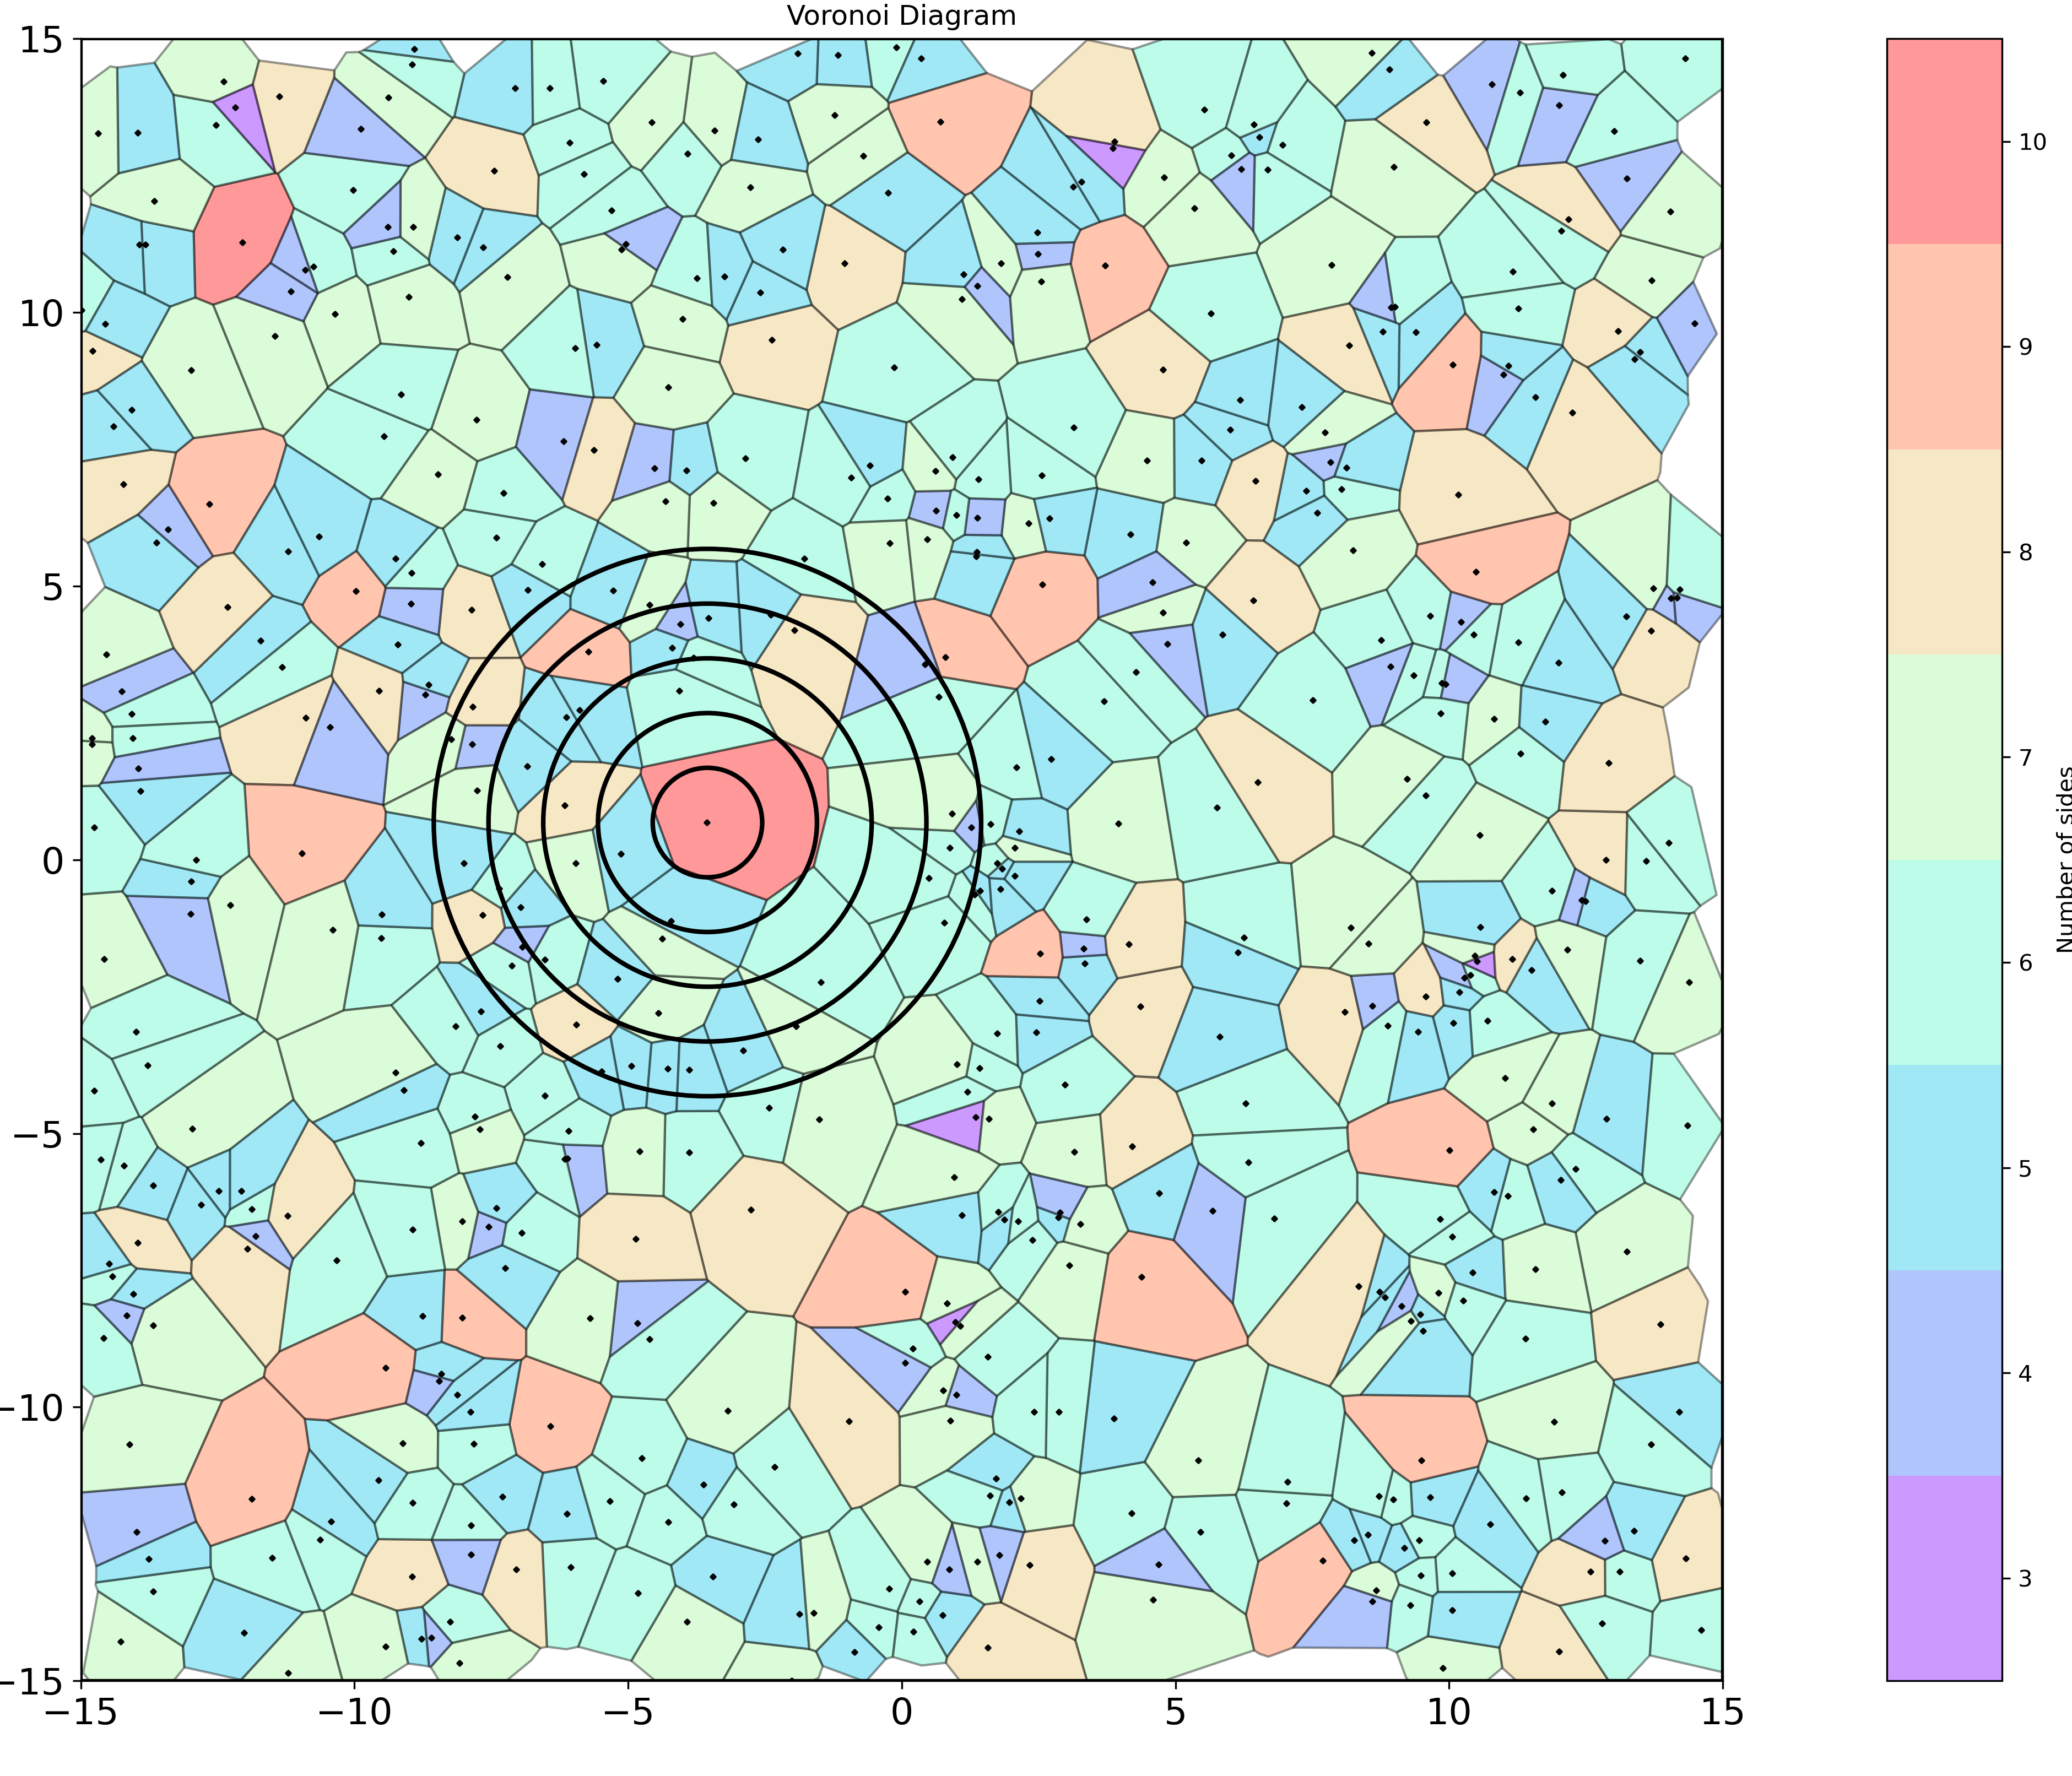
\includegraphics[width=0.8\linewidth]{figures/crystalline_voronoi_d_cut_circles.png} 
  \caption{dcut visual}
  \label{fig:dcut}
\end{figure}


\subsubsection{Reorganization energy}
Marcus's nonadiabatic electron transfer theory allows us to model charge transfer as two
intersecting parabolic potential energy surfaces. In this work, the parabalas represent the potential energy surface
of the dimer created by a pair of chomophores with a charge injected on either chromophore. In this context, 
reorganization energy, $\lambda_{ij}$, constitutes the energy required to distort the dimer's equilibrium geometry with a
charge on chromophore $i$ into the dimers equillibrium geometry with charge on chromophore $j$.
Reorganization energy consist of the energy change associated with the destortion of the dimers geometry,
and the distortion of the surrounding medium in responce the movement of the charge. It can be written as
follows:
\begin{align}
    \lambda_{total} = \lambda_{internal} + \lambda_{external}.
\end{align} 
$\lambda = 0.3eV$ is chosen to be the default reorganization energy ($\lambda_{internal} = 0.1eV$
and $\lambda_{external} = .02eV$) as others have done with P3HT \cite{jones2017} and
a flourene-triphenylamine copolymer, TFB \cite{Gali2017}. 

\begin{figure}
  \center
  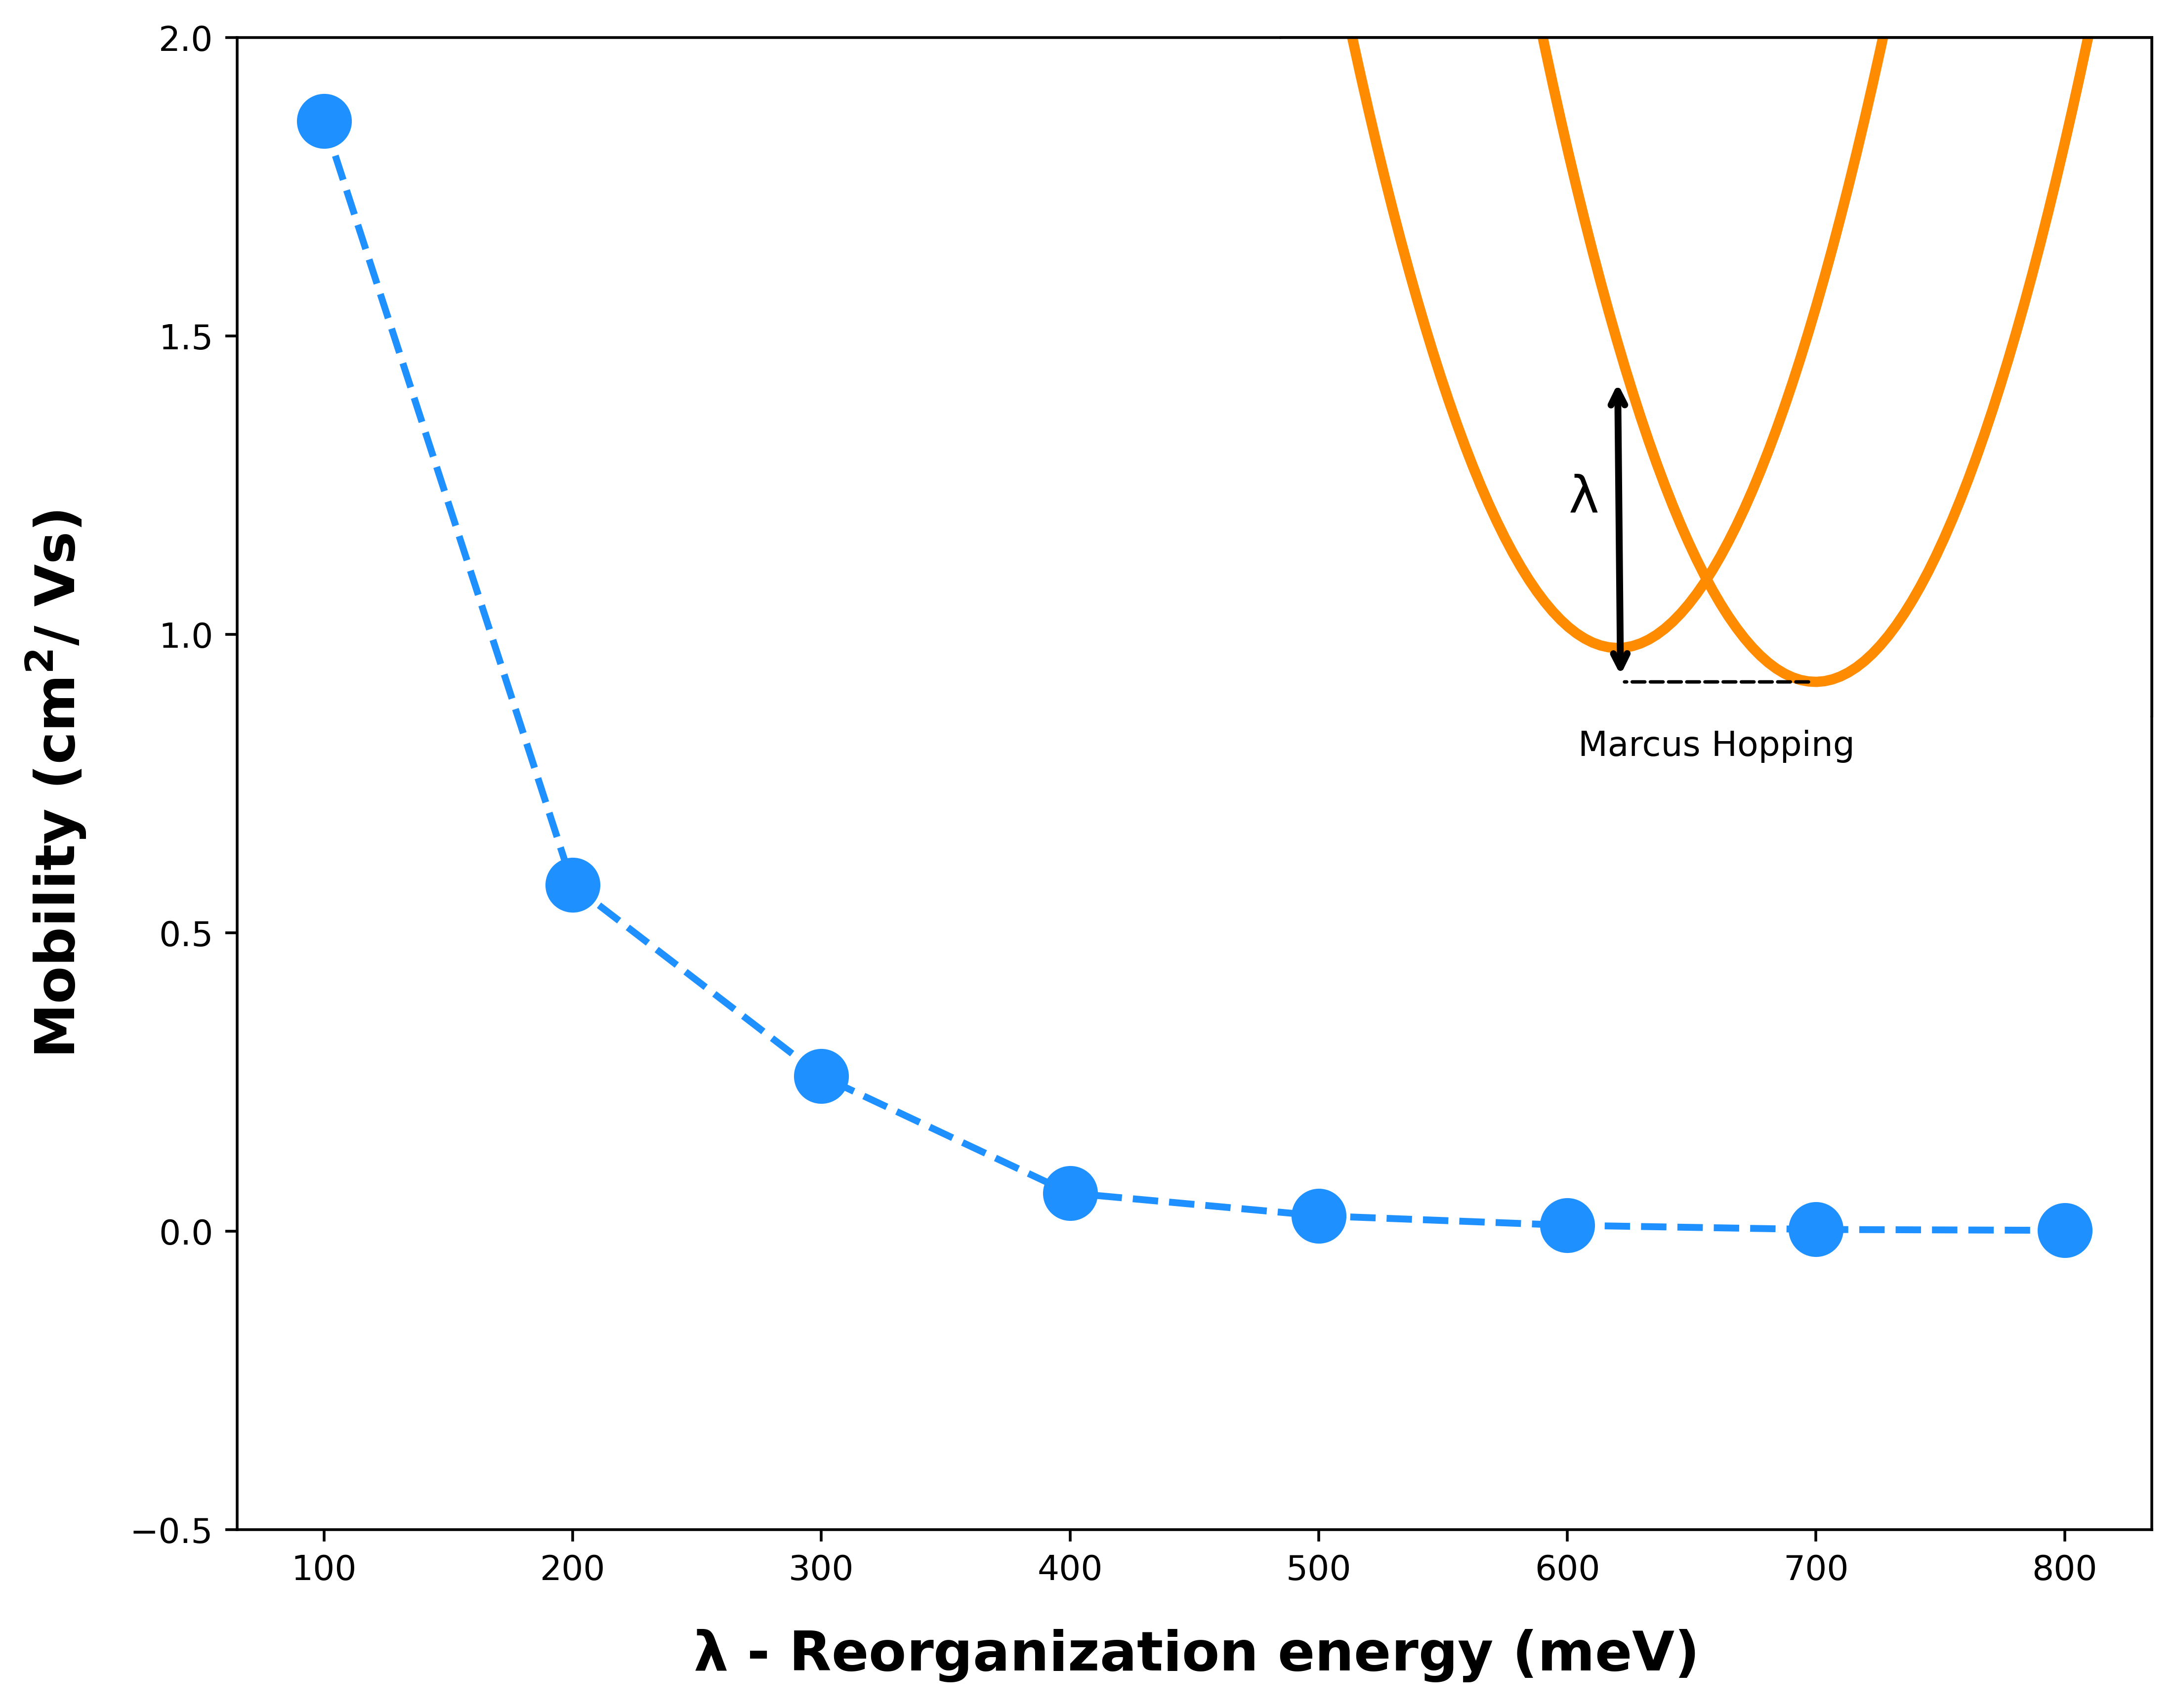
\includegraphics[width=0.8\linewidth]{figures/reorg.png} 
    \caption{The results of running 8 KMC simulations with reorganization energy 100-800 meV}
  \label{fig:reorg}
\end{figure}

\subsubsection{Temperature}

Another parameter of interest in the Marcus theory mention above is temperuture. To test the sensitivity to
temperature, 15 KMC simulations from 100K to 800k were run on the benchmark P3HT crystalline morphology. It
is clear from the results in [FIGURE] that the mobilities trend upward with temperature. With relatively
weak electronic coupling ($T_{ij}$) between chromophores, electron transfer proceeds nonadiabatically
\cite{clarke2010}. With this weak coupling, the temperature in the Gibbs free energy of activation term
dominates the effect temperature has hop rate. 

\begin{figure}[]
\centering
\begin{subfigure}{.5\textwidth}
    \textbf{(A)}
    \centering
    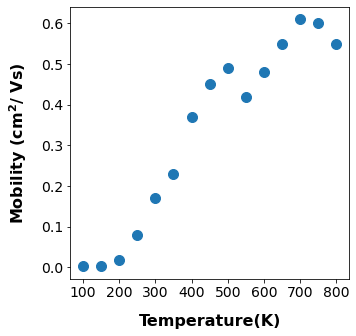
\includegraphics[width=\textwidth]{figures/temp.png}
    \newline
\end{subfigure}%
\begin{subfigure}{.5\textwidth}
    \textbf{(B)}
    \centering
    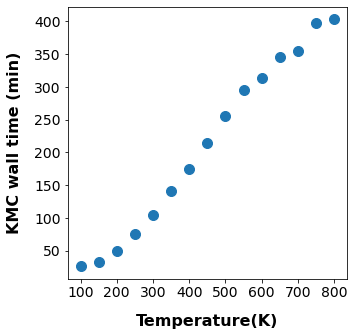
\includegraphics[width=\textwidth]{figures/temp_simtime_plot.png}
    \newline
\end{subfigure}
\begin{subfigure}{.5\textwidth}
    \textbf{(C) 100K}
    \centering
    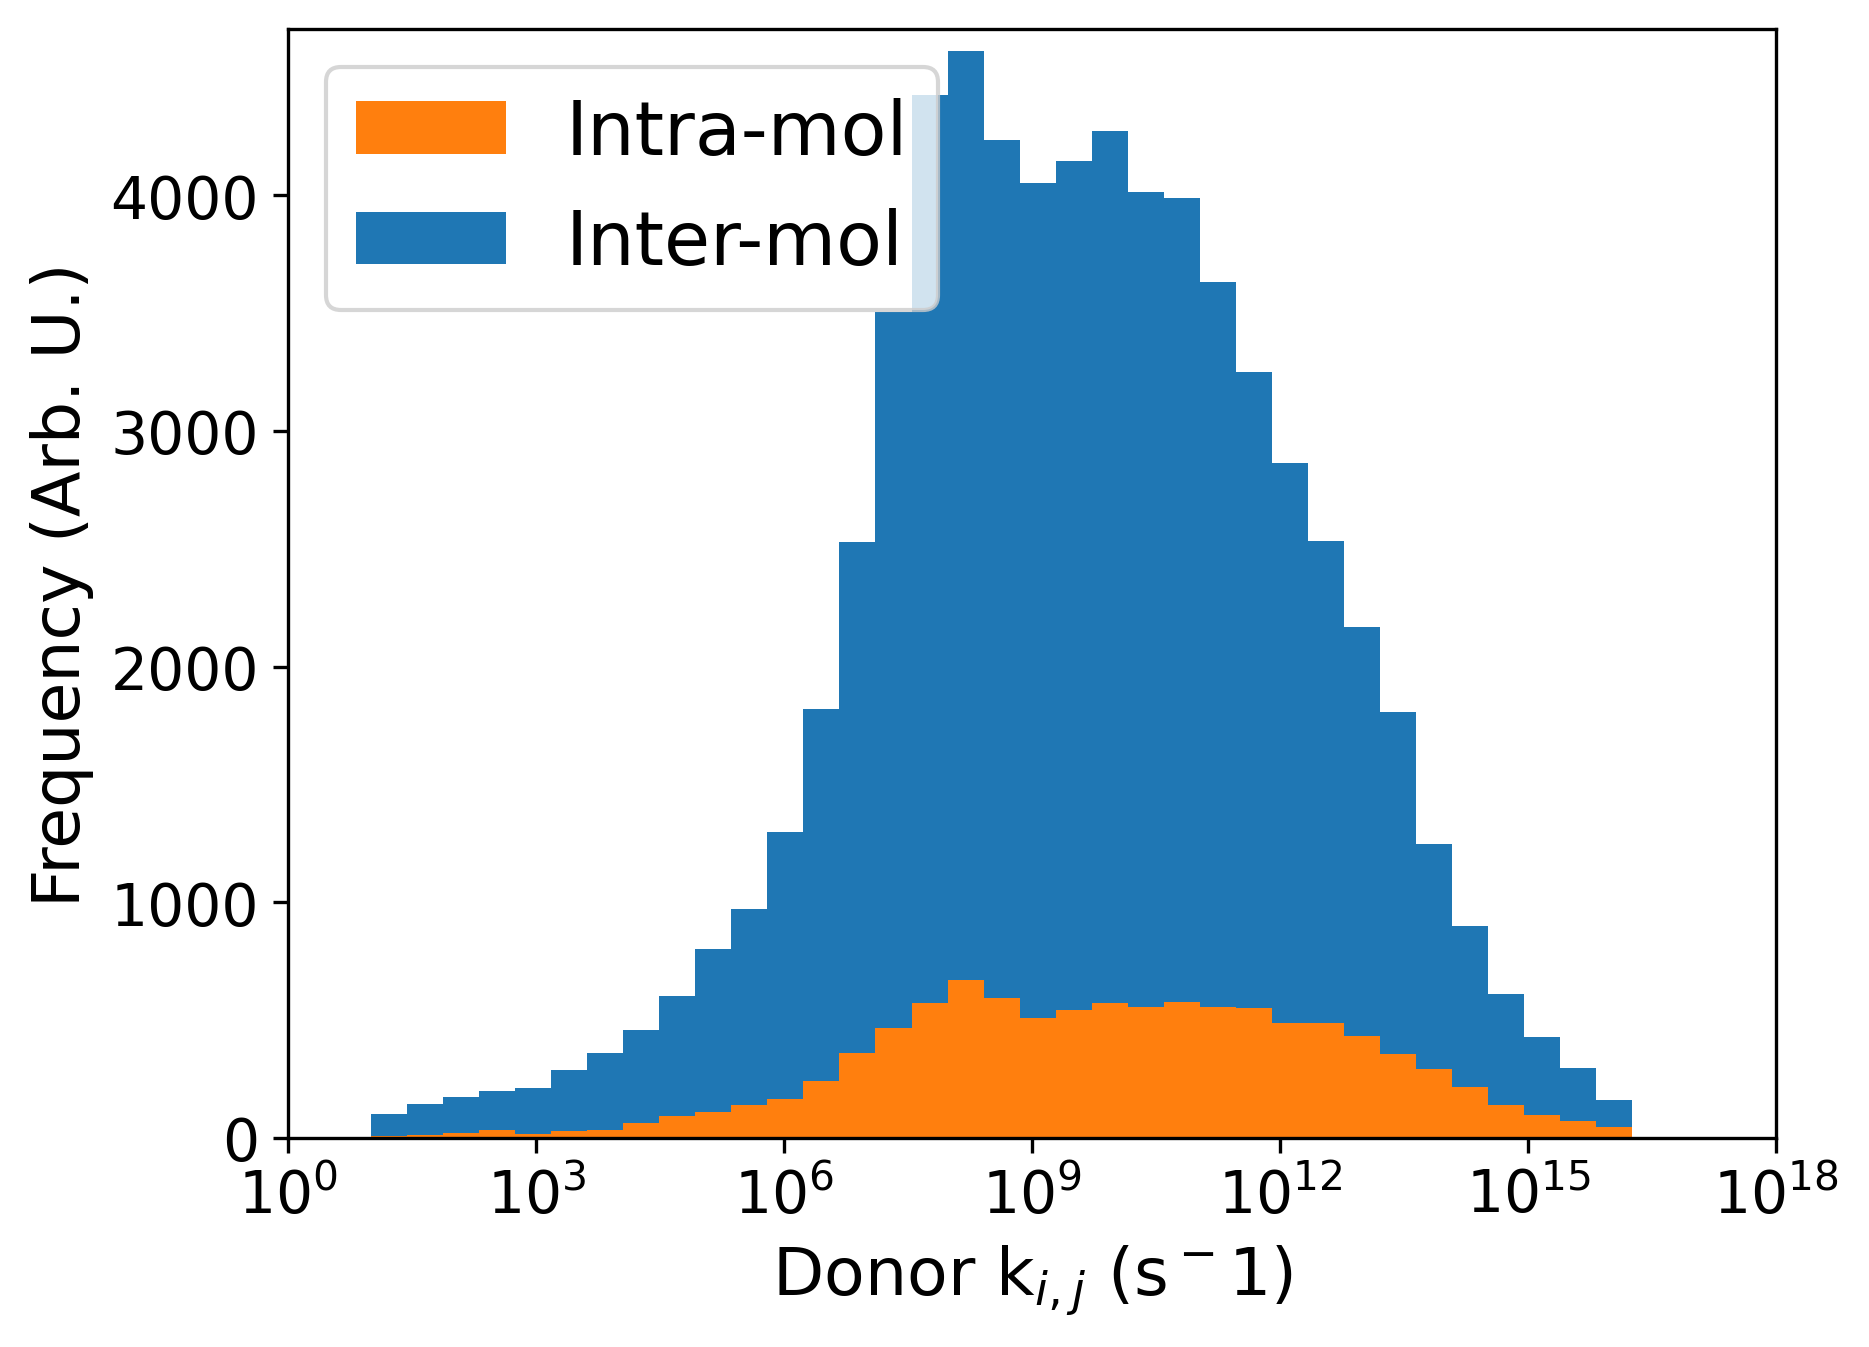
\includegraphics[width=\textwidth]{figures/donor_hopping_rate_clusters_temp100.png}
\end{subfigure}%
\begin{subfigure}{.5\textwidth}
    \textbf{(D) 800K}
    \centering
    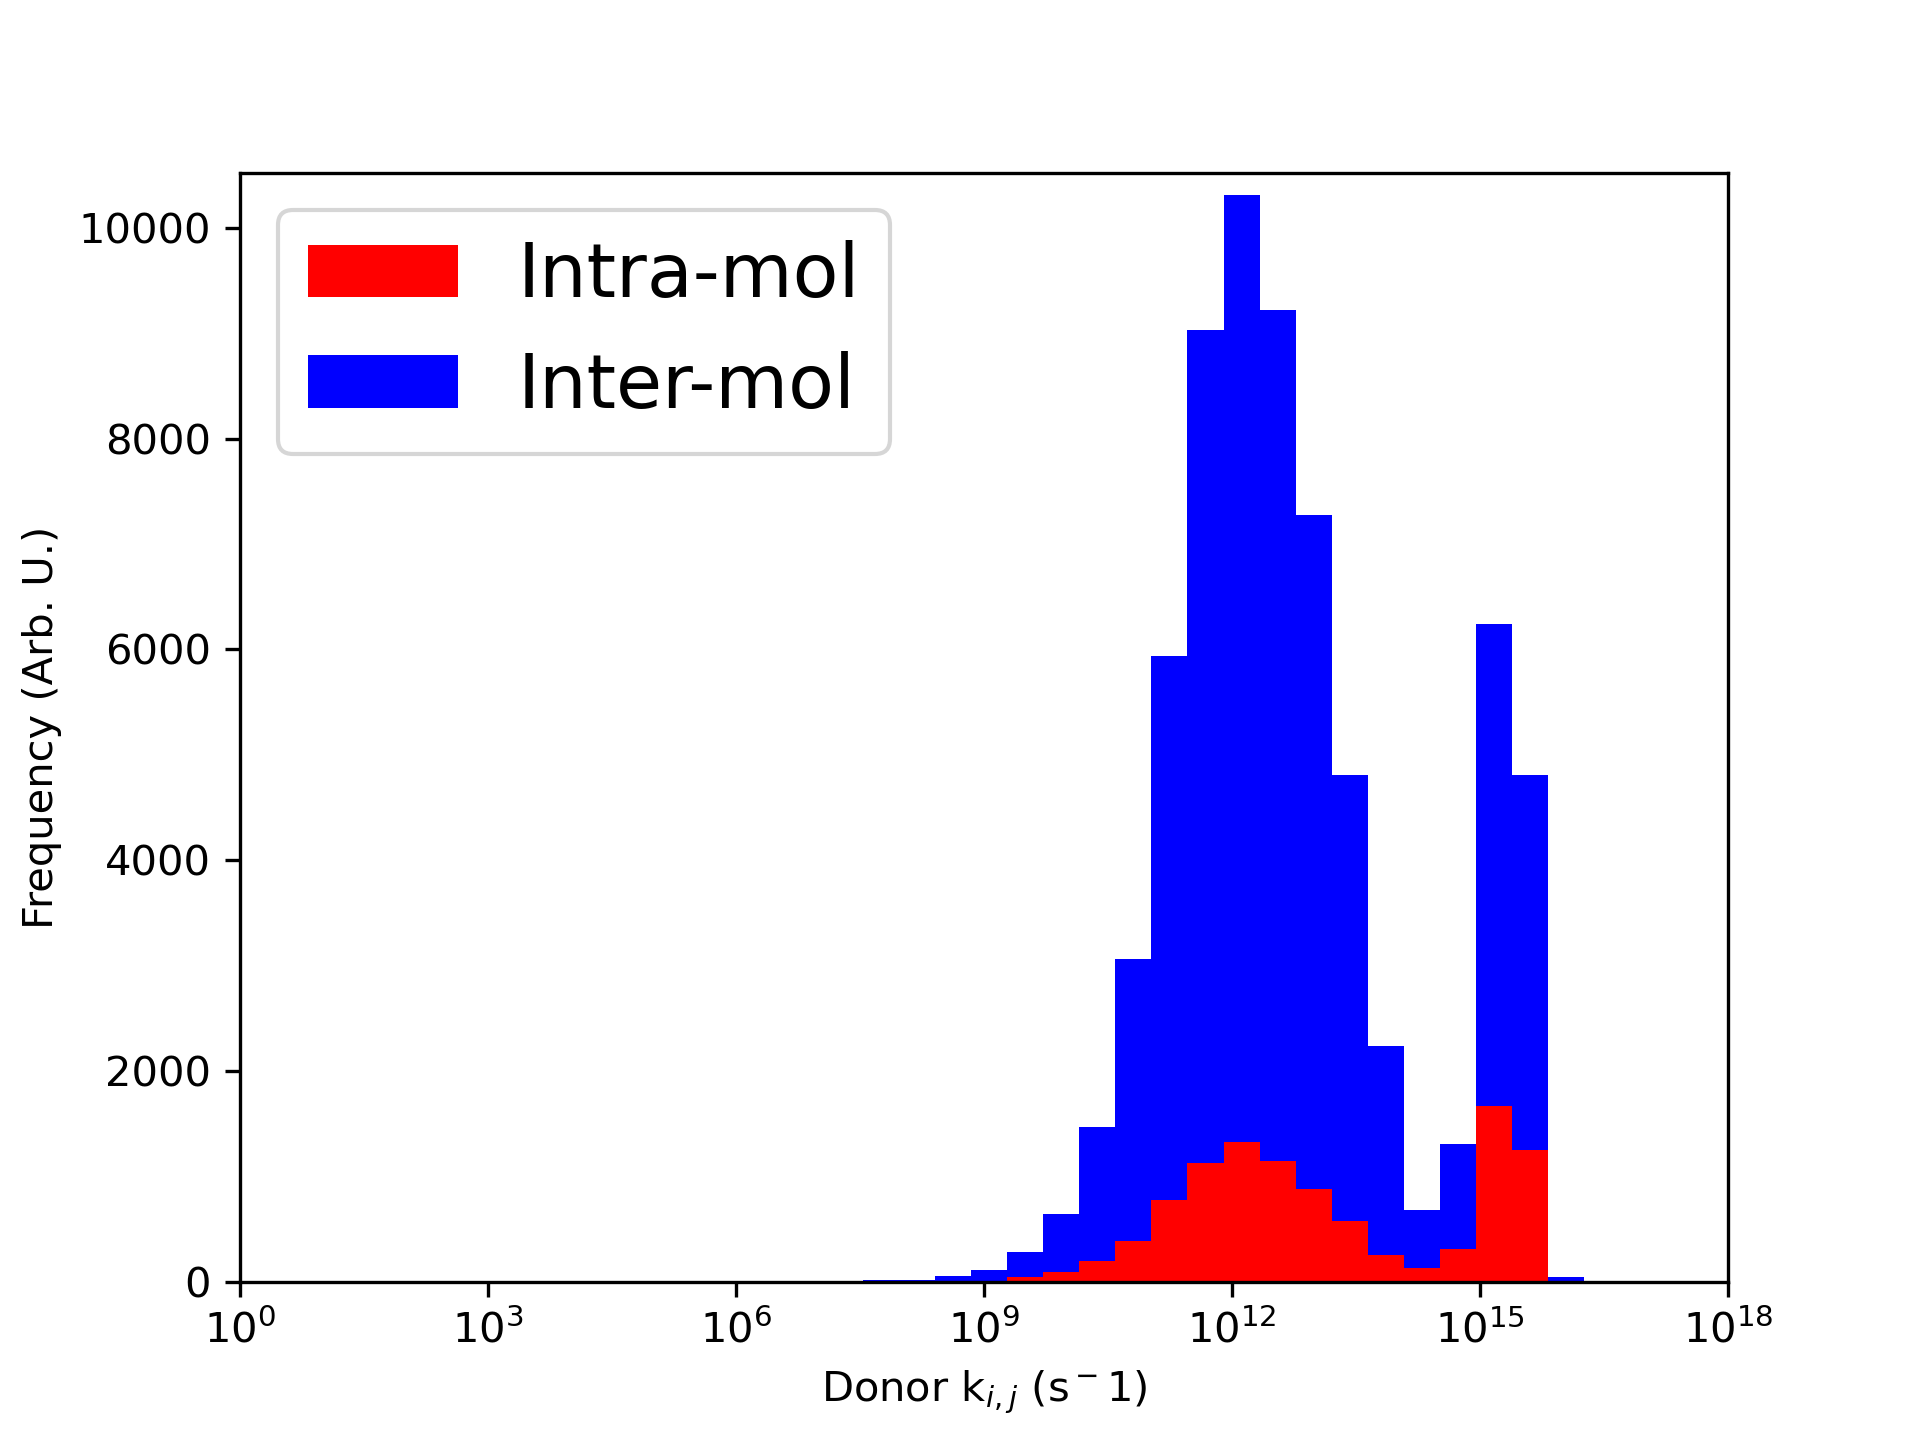
\includegraphics[width=\textwidth]{figures/donor_hopping_rate_clusters_temp800.png}
\end{subfigure}
\caption[short]{A beautiful, well written caption}
\end{figure}

\subsubsection{lifetimes}
The KMC algorithm allows an explicit calculation of the MSD accross a large number of 
particles in the system. Repeating along relevant time scales for 
charge transfer, the slope of this relationship
can be estimated and related to to the 3D diffusion coeffiecient as discussed in the methods section of this
work. Using the Einstien relation (2.3), 
the groundwork for which Einstein derived in his doctoral dissertaion, finally the zero-field
mobility can be obtained. 
It is critical that we not include the ballistic transport timescale in the approximation of the limit
if the slope as time goes to infinity \cite{Maginn2018}. Estimating an upperbound for lifetimes such that
we can estimate the slope of the MSD as time goes to infinity can be messy. In real systems, free chrage
carrier lifetime is subject to a complex interplay between geminate recombination, non-geminate recombination,
charge trapping, temperature, and charge density, whose dynamics play out accros a picosecond to microsecond
timescales and vary widly form material to material as well as from microstrtucture to microstrucute for a
given material \cite{Laquai2015} . For this work, the primary strategy was to avoid the ballistic region while exploring lifetimes
that are achievable computationally. For example, in an attempt to simulate out to the physical limit, a
simulation a microsecond($10^{-6} seconds$) lifetime resulted in a single hole hopping for 9 wall time hours.
It is advised that a preanalysis to determine where a given morphology's MSD will convergeb be performed so as
to never simulate past that point. Doing so is superflous and could introduce unessacery noise into the data. 
\subsection{ITIC}
To explore the extensibility of the workflow on another benchmark OPV material, using planckton-flow, a 1000
molecule morphology of ITIC was equillibrated over 10e-7 frames of an MD simulation. The the reported
experimental electron mobility of ITIC varies depending on how it was processed and how it was measured. A
time-of-flight electron mobilities on the order of $10^{-4}$ \cite{Mica2018} and field effect mobilities on the order of
$10^{-2}$ \cite{Park2018} have been reported. 

\subsection{Improvements}
In this work, we ignore dynamic disorder by doing calculations on snapshots from equillibrium MD simulations.
Others have had success intruducing dynamic disorder via nudging the QQC calculated TI value at every
iteration of the KMC algorithm by a number drawn randomly from a Gaussian Distribtion \cite{Gali2017}.

Dynamic disorder does effect charge mobility (CT in high mobility conjugated polymers) with every pico second
may have a 10-20\% fluxuation in TI. Need to find the paper but using the dynamic dimer methor for TI calc
could be a way to introduce dynamic disorder. Or it could be done as mentioned before in another paper where
they use two different methods one with a guassians fluxuation and sime ohther fancy method. 

In our kmc algorithm we could incorperate the rates of other events like recombination.

The computational bottle neck of simulation charge mobility is also the most theoreticaly challenging.
Estimating the TI for each pair of cromophores. A future improvement to MorphCT will be accelerating this step
with Machine learning techniques. Musil et al. have shown that ML could produce a 90 \% decrease in
computationl effort \cite{Musil2018}

Something to do is allow morphct as to figure out what to do with donor accpeter mixtures. It would be pretty
easy to run asyncronously on the donor/acceptor materials and compare. this could be a measure of morphology.
If you run pure donor and pure acceptor and you got mobities, if on of those drops in the mixed morph more
that the other you probably dont have a nice domain for BHJ.

%%% Local Variables: 
%%% mode: latex
%%% TeX-master: "BSUmain"
%%% End: 
